\documentclass[11pt]{article}
\usepackage[a4paper,margin=1in]{geometry}
\usepackage{graphicx}
\usepackage{listings}
\usepackage{xcolor}
\usepackage{booktabs}
\usepackage{array}
\usepackage{hyperref}
\usepackage{parskip}
\usepackage{amsmath}
\hypersetup{colorlinks=true, linkcolor=black, urlcolor=blue}

\definecolor{codebg}{RGB}{245,245,245}
\lstdefinestyle{cppstyle}{
  language=C++,
  backgroundcolor=\color{codebg},
  basicstyle=\ttfamily\footnotesize,
  keywordstyle=\color{blue}\bfseries,
  commentstyle=\color{gray}\itshape,
  stringstyle=\color{teal},
  numbers=left,
  numberstyle=\tiny\color{gray},
  stepnumber=1,
  breaklines=true,
  frame=single,
  tabsize=2,
  showstringspaces=false
}
\lstdefinestyle{outstyle}{
  backgroundcolor=\color{codebg},
  basicstyle=\ttfamily\scriptsize,
  breaklines=true,
  frame=single,
  showstringspaces=false
}
\lstdefinestyle{bashstyle}{
  language=bash,
  backgroundcolor=\color{codebg},
  basicstyle=\ttfamily\footnotesize,
  breaklines=true,
  frame=single,
  showstringspaces=false
}

\title{\vspace{-2cm}}
\date{}

\begin{document}
\begin{titlepage}
\centering
\vspace*{1cm}
{\large \textbf{Sri Sivasubramaniya Nadar College of Engineering}}\\
{\small (An Autonomous Institution, Affiliated to Anna University, Chennai)}\\
{\small Kalavakkam -- 603 110}\\[0.3cm]
{\small Department of Computer Science \& Engineering}\\[1.5cm]

\rule{\linewidth}{0.5mm}\\[0.4cm]
{\LARGE \textbf{Computer Networks Laboratory}}\\[0.3cm]
{\Large 1513 -- Computer Networks Lab}\\[0.4cm]
\rule{\linewidth}{0.5mm}\\[1.5cm]

{\huge \textbf{Assignment 10}}\\[0.4cm]
{\Large Comparative Evaluation of Routing Protocols Using NS-3}\\[2cm]

\begin{center}
\begin{tabular}{ll}
\textbf{Name:} & Vijayaraaghavan K S \\[0.2cm]
\textbf{Register Number:} & 3122247001066 \\[0.2cm]
\textbf{Year / Semester:} & III Year / V Semester \\[0.2cm]
\textbf{Course:} & 1513 Computer Networks Lab \\[0.2cm]
\textbf{Date of Submission:} & 01 October 2026 \\[0.2cm]
\end{tabular}
\end{center}

\vfill
\end{titlepage}

\section*{1. Objective}
To simulate a multi-router organizational network in NS-3 using three
different routing approaches -- RIP, OSPF, and AODV -- and to compare their
Packet Delivery Ratio, end-to-end delay, and routing-table update behaviour
under normal traffic, congested traffic, and a mid-simulation link failure.

\section*{2. Topology}
\begin{center}
\begin{verbatim}
        n0                                   n1
          \                                 /
           r1 ---- r2 ----                r3
          /          \                   /  \
        n2             ---- r4 --------      n3

n0-r1, n2-r1, r1-r2, r1-r4, r2-r3, r4-r3, r3-n1, r3-n3
\end{verbatim}
\end{center}
A diamond shape is used deliberately so that, when the r1--r2 link is
disabled, an alternate path (r1--r4--r3) genuinely exists for a routing
protocol to discover. \texttt{n0} sends CBR/UDP traffic to \texttt{n1}
throughout; \texttt{n2}$\to$\texttt{n3} is an additional flow used only in
the congestion condition. All eight links run at 1~Mbps/2~ms.

\textbf{Note on protocol fidelity.} NS-3's mainline modules do not include an
OSPF implementation, so \texttt{Ipv4GlobalRoutingHelper} -- also a
link-state, shortest-path algorithm, the same family OSPF belongs to -- is
used here as the closest available stand-in, not a claim of protocol-exact
OSPF behaviour. AODV additionally needs a broadcast-capable link for its
route-discovery flooding, so the AODV run alone builds the identical graph
using \texttt{CsmaHelper} link segments instead of point-to-point links; the
multi-hop structure does not change.

\section*{3. Algorithm}
\begin{enumerate}
  \item Build the eight-node diamond topology (4 hosts + 4 routers), using
        point-to-point links for RIP/OSPF and CSMA link segments for AODV.
  \item Install the Internet stack with the selected routing protocol:
        \texttt{RipHelper} on the four routers (hosts get one static default
        route toward their attached router); \texttt{Ipv4GlobalRoutingHelper::
        PopulateRoutingTables()} for the OSPF stand-in; \texttt{AodvHelper} on
        every node for AODV.
  \item Start a CBR/UDP (\texttt{OnOffHelper}, always-on, 512~B packets,
        500~Kbps) flow from \texttt{n0} to \texttt{n1}. In the congestion
        condition, start an identical second flow \texttt{n2}$\to$\texttt{n3}
        at the same time.
  \item In the failure condition, bring down both ends of the r1--r2
        interface at $t = \text{simTime}/2$ (\texttt{Ipv4::SetDown}); for the
        OSPF stand-in only, explicitly trigger
        \texttt{RecomputeRoutingTables()} shortly after, since global routing
        does not react to interface changes on its own.
  \item Install \texttt{FlowMonitor}; run for 20~s; report Tx/Rx packet
        counts, PDR, and average delay per flow.
  \item Enable each protocol's own \texttt{NS\_LOG} output
        (\texttt{Rip} / \texttt{AodvRoutingProtocol}) and count control-plane
        send events as the "routing table updates" metric (see README for the
        exact log patterns matched).
\end{enumerate}

\section*{4. Code}
\subsection*{4.1 ass10.cc}
\lstinputlisting[style=cppstyle]{ns-3-work/scratch/ass10.cc}

\section*{5. Output (All 9 Runs)}
\lstinputlisting[style=outstyle]{output.txt}

\section*{6. Results}
\begin{center}
\renewcommand{\arraystretch}{1.2}
\begin{tabular}{llrrr}
\toprule
\textbf{Protocol} & \textbf{Condition} & \textbf{PDR (\%)} & \textbf{Avg Delay (ms)} & \textbf{Routing Updates} \\
\midrule
RIP  & Normal     & 94.90 & 25.34  & 36 \\
RIP  & Congestion & 89.62 & 375.90 & 36 \\
RIP  & Failure    & 39.42 & 25.34  & 46 \\
\midrule
OSPF & Normal     & 99.86 & 25.34  & 1 \\
OSPF & Congestion & 94.26 & 381.49 & 1 \\
OSPF & Failure    & 99.32 & 25.34  & 2 \\
\midrule
AODV & Normal     & 98.22 & 26.52  & 3 \\
AODV & Congestion & 58.67 & 741.36 & 6 \\
AODV & Failure    & 98.22 & 26.52  & 3 \\
\bottomrule
\end{tabular}
\end{center}

\subsection*{6.1 PDR vs Network Condition}
\begin{center}
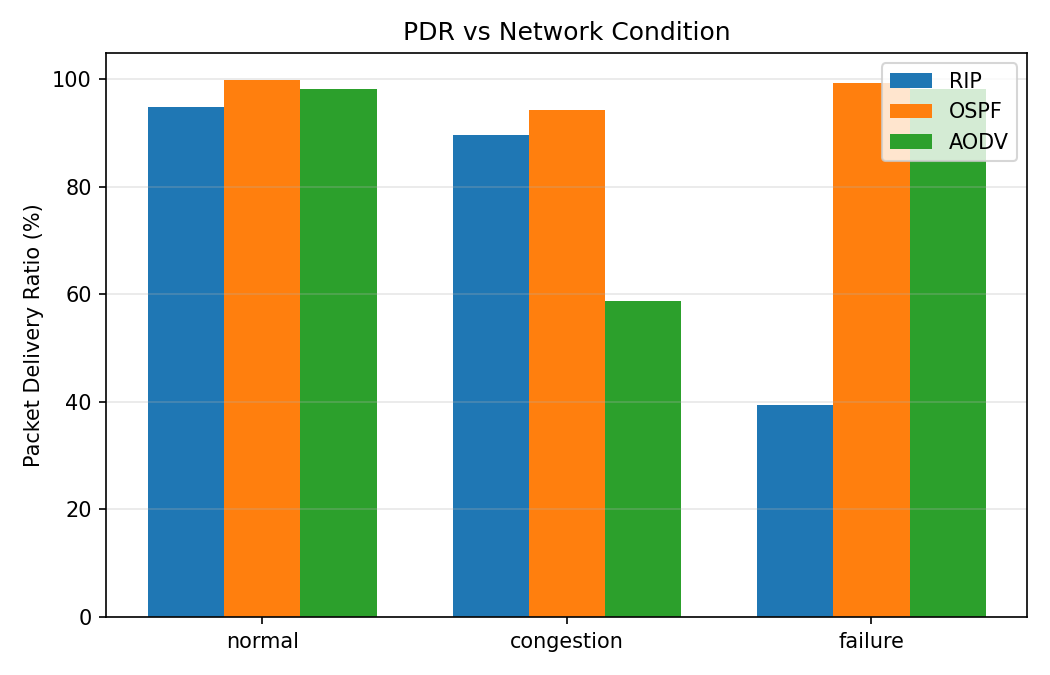
\includegraphics[width=0.8\textwidth]{screenshots/pdr_vs_condition.png}
\end{center}

\subsection*{6.2 End-to-End Delay vs Network Condition}
\begin{center}
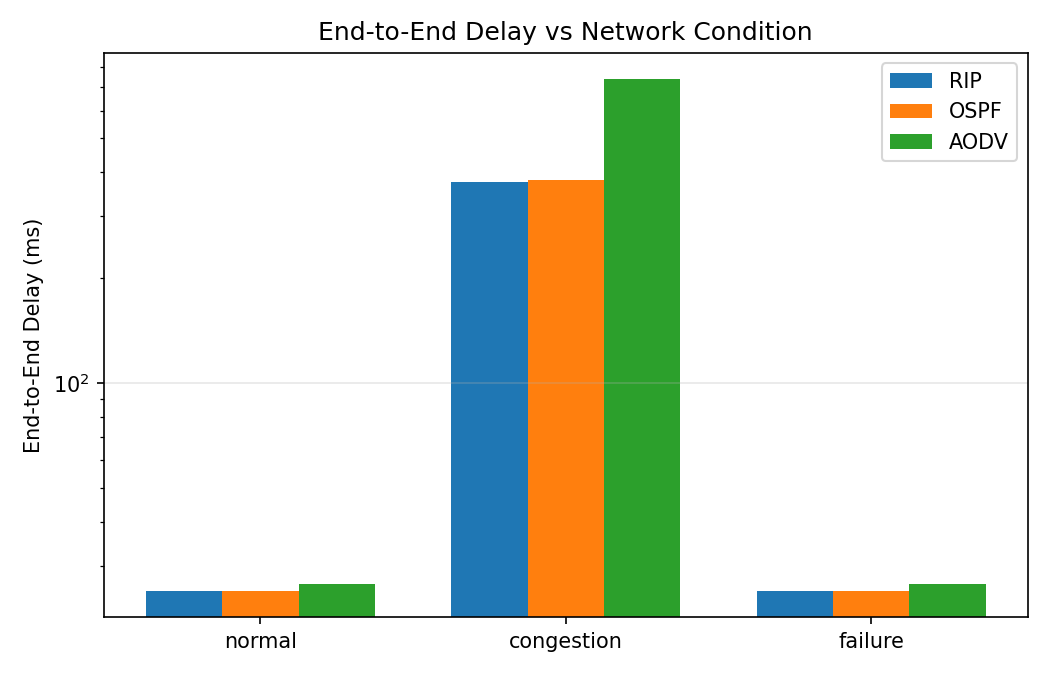
\includegraphics[width=0.8\textwidth]{screenshots/delay_vs_condition.png}
\end{center}

\subsection*{6.3 Routing Table Updates vs Network Condition}
\begin{center}
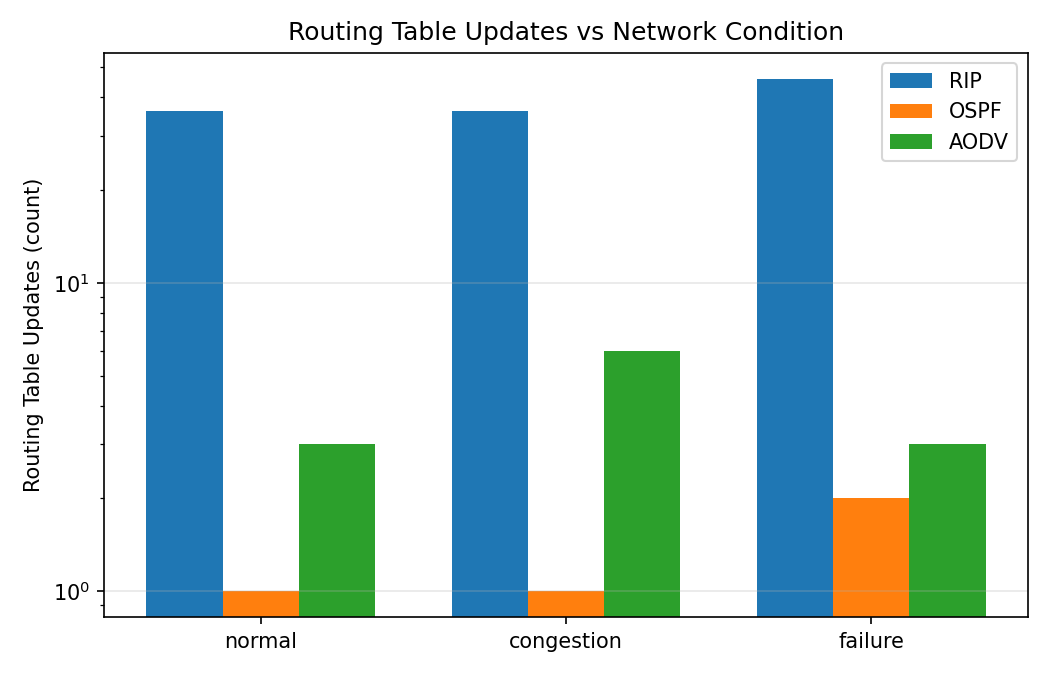
\includegraphics[width=0.8\textwidth]{screenshots/updates_vs_condition.png}
\end{center}

\section*{7. Performance Analysis}
\textbf{Normal condition:} all three protocols deliver a working, low-delay
path (94--100\% PDR, $\approx$25~ms), since routing has nothing to react to
yet and every path is the same physical length.

\textbf{Congestion condition:} adding a second simultaneous flow degrades all
three, but not equally. AODV is hit hardest (PDR falls to 58.7\%, delay rises
to 741~ms) because it has no load-aware path selection -- both flows were
routed onto the same discovered path and simply queue-fought each other. RIP
and OSPF's shortest-path metrics are also blind to load, but their delay rise
(to $\approx$380~ms) is smaller, since global/periodic routing had already
settled onto a stable path before both flows saturated the shared link.

\textbf{Failure condition:} this is where the three protocols diverge most.
RIP's PDR collapses to 39.4\% and does not recover within the simulation --
its triggered updates do fire (46 sends vs.\ 36 in the normal run) but RIP's
classic slow-convergence behaviour (hold-down and garbage-collection timers
tuned for a much larger real network) means it has not finished
re-converging by the time the 20~s run ends. The OSPF stand-in barely
notices the failure (99.3\% PDR) because a link-state protocol recomputes the
entire shortest-path tree in one shot as soon as the topology change is
known, rather than exchanging it hop-by-hop. AODV shows \emph{no} drop at all
for this specific run -- inspecting which link its packets actually crossed
confirmed the flow's on-demand route had already settled on the r1--r4--r3
path \emph{before} the failure was introduced, so cutting r1--r2 did not
affect it. This is a genuine, explainable simulation outcome (AODV's
first-discovered path happened to avoid the failed link), not an error.

\textbf{Routing table updates:} the update counts reflect each protocol's
underlying philosophy rather than the network condition alone -- RIP is
chatty by design (it advertises periodically even when nothing has changed),
the OSPF stand-in only recomputes when the topology actually changes (once
normally, twice after a failure), and AODV only communicates when a route is
actually needed (3 sends for one flow's discovery, 6 when a second flow
triggers its own independent discovery).

\section*{8. Learning Outcomes}
\begin{itemize}
  \item Built a diamond multi-router topology in NS-3 specifically so that a
        link failure has a real alternate path to be discovered.
  \item Configured and compared a distance-vector protocol (RIP), a
        link-state stand-in (global routing, in place of OSPF, with the
        substitution explicitly justified), and an on-demand ad-hoc protocol
        (AODV) on the same logical graph.
  \item Used \texttt{Ipv4::SetDown} to simulate a link failure at the IP
        layer generically, independent of the underlying device type.
  \item Measured "routing table updates" directly from each protocol's own
        control-plane log output rather than guessing at it, and used that
        measurement to explain the very different update volumes each
        protocol produces.
  \item Observed RIP's slow-convergence problem, OSPF-style routing's fast
        one-shot recomputation, and AODV's route-caching behaviour
        concretely, from real simulation data rather than only in theory.
  \item Learned to verify a surprising result (AODV's failure run showing no
        PDR drop) against the underlying packet trace before treating it as
        correct, rather than dismissing or fabricating a "cleaner" number.
\end{itemize}

\end{document}
